\documentclass[10pt,letterpaper]{article}
\usepackage{neurips_2024}

\usepackage{xspace}
\usepackage{url}
\usepackage{amsmath}
\usepackage{booktabs}
\usepackage{tabularx}
\usepackage{multirow}
\usepackage{makecell}
\usepackage{enumitem}
\usepackage{listings}
\usepackage{parskip}
\usepackage{float}
\usepackage{tikz}
\usetikzlibrary{arrows.meta, positioning, shapes.geometric}

\setlength{\parskip}{4pt}
\setlength{\parindent}{12pt}
\setlength{\emergencystretch}{2em}

\newcommand{\gridcast}{\textsc{GridCast}\xspace}
\newcommand{\graphcast}{\textsc{GraphCast}\xspace}
\newcommand{\gencast}{\textsc{GenCast}\xspace}
\newcommand{\tft}{\textsc{TFT}\xspace}
\newcommand{\eg}{\textit{e.g.,}\xspace}
\newcommand{\ie}{\textit{i.e.,}\xspace}

% ============================================================
\title{GridCast: Design Document \& Implementation Plan}

\subtitle{Amendment to the Project Proposal $\vert$ Draft for Team Review}

\author{%
  \textit{[Author names omitted for review]}
}

\date{}

% ============================================================
\begin{document}

\maketitle

% ============================================================
\begin{abstract}
This document extends the original \gridcast proposal with three additions: (1) corrections
and clarifications to the original proposal where assumptions required revision; (2) a
concrete user story defining who interacts with the system and how; and (3) a full
implementation design covering the machine learning architecture, technology stack,
infrastructure plan, and phased build sequence. The target artefact is a live,
interactive hackathon demo deployable on IBM Cloud within a \$100 budget, targeting
the IBM Technologies integration prize.
\end{abstract}

% ============================================================
\section{Amendments to the Original Proposal}

The original proposal is technically sound in its framing and data sourcing strategy.
Three points require clarification or amendment before implementation begins.

\subsection{GenCast Compute Requirements}

The original proposal presents \gencast as a freely runnable inference layer.
In practice, \gencast requires TPU infrastructure to generate the 50-member ensemble at
meaningful scale. At cloud GPU rates (approximately \$3--6 per run on an A100), a handful
of demonstration runs are feasible within budget, but continuous inference is not.

\textbf{Demo resolution:} The live demonstration will use the
\textbf{Open-Meteo Ensemble API} as the probabilistic weather source. Open-Meteo provides
a 16-member GFS ensemble at no cost, no API key required, with a 10-day forecast horizon
at hourly resolution --- sufficient to drive the probabilistic pipeline. In the pitch and
accompanying materials, \gencast is presented as the production upgrade path with full
narrative continuity.

\subsection{ML Model Specification}

The original proposal describes a ``weather-to-grid-stress mapping'' without specifying
the model architecture. This is the core ML contribution and requires a concrete choice.

\textbf{Selected model:} A \textbf{Temporal Fusion Transformer} (\tft), implemented
via the \texttt{pytorch\discretionary{-}{}{-}forecasting} library. The \tft was chosen for three reasons: it
handles multi-horizon forecasting natively (up to 240 hours / 10 days), it accepts mixed
tabular and temporal inputs matching the three-layer feature matrix, and it produces
native output quantiles without post-hoc calibration. The quantile outputs directly
populate the fan chart bands in the user interface.

\subsection{Live Inference vs.\ Backtesting}

The original proposal conflates validation (backtesting on historical stress events)
with real-time operation (hourly contract triggers). These are distinct modes.

\textbf{Clarification:} The model is \emph{trained offline} on historical data.
``Live'' in the demo context means: at demo time, the system fetches today's real EIA
demand data and today's real Open-Meteo ensemble forecast, runs inference against the
trained model, and updates the map in real time. The model is not re-trained live.
The three historical stress events (Texas 2021, Pacific Northwest 2022, PJM Summer 2023)
serve as a \emph{stress event replay} mode in the UI, showing what the forecast would
have looked like 10 days before each event occurred.

% ============================================================
\section{User Story}

\subsection{Product Tiers}

\gridcast is designed in two tiers with distinct users.

\paragraph{Tier 1 --- Demo \& Investor View (hackathon target).}
The audience is investors, judges, and potential utility partners evaluating the concept.
The interface is a public US map showing the transmission nodes under observation,
colour-coded by current stress probability. A visitor clicks a node and immediately sees
a 10-day probabilistic forecast, the current recommended power allocation percentage,
and a set of simulated data centre neighbours with their assigned draw percentages.
This tier uses exclusively public data and requires no access agreement with any utility.

\paragraph{Tier 2 --- Operator-Facing Dashboard (production path).}
Once a utility or grid operator licenses the product and provides internal SCADA or
settlement data, the interface shifts from the public map to an internal operations view
showing the utility's own grid topology, real transmission node identifiers, live
metering data, and contractual commitment windows. The operator persona is a grid
reliability engineer or demand response manager who runs a 10-day forecast each morning
and uses it to decide which flexible contracts to trigger, how much capacity to commit to
data centre tenants, and when to issue curtailment notices.

\subsection{Core User Interaction --- Tier 1}

The canonical user action for the demo proceeds as follows:

\begin{enumerate}[leftmargin=*, label=\arabic*.]
  \item The user opens the web application and sees a full US map with four highlighted
        transmission nodes.
  \item Each node displays a colour indicator (green / amber / red) driven by the
        current 24-hour peak stress probability from the model.
  \item The user clicks the \textbf{Dominion Hub} node (Northern Virginia).
  \item A side panel opens showing: the 10-day forecast fan chart, the current LMP
        congestion value, the EIA demand deviation (actual vs.\ forecast), and the
        headline recommended allocation percentage with its confidence band.
  \item The panel also shows three simulated data centres nearby, each assigned a
        draw percentage for today derived from the allocation output.
  \item The user clicks \textbf{``Refresh Forecast''}. The backend fetches the latest
        EIA hourly reading and the latest Open-Meteo ensemble, reruns inference, and
        the chart updates visibly.
  \item The user selects \textbf{``Replay: Texas Winter Storm 2021''} from a dropdown.
        The map transitions to a replay view showing the forecast as it would have
        appeared on 1 February 2021 --- 10 days before the storm peak. The fan chart
        shows the growing uncertainty band as the horizon extends, illustrating exactly
        the utility of confidence bounds.
\end{enumerate}

% ============================================================
\section{Target Nodes}

Four transmission nodes are selected for the demonstration, covering three ISOs and two
California zones. Table~\ref{tab:nodes} lists the nodes, their rationale, and their
data sources.

\begin{table}[H]
\centering
\caption{Target transmission nodes for the GridCast demo.}
\label{tab:nodes}
\renewcommand{\arraystretch}{1.3}
\begin{tabularx}{\linewidth}{@{}llllX@{}}
\toprule
\textbf{Node} & \textbf{ISO} & \textbf{State} & \textbf{EIA BA} & \textbf{Narrative} \\
\midrule
Dominion Hub   & PJM    & Virginia       & PJM  & Largest US data centre corridor;
                                                   \$38.70/MWh congestion case in
                                                   proposal Appendix~A \\
CAISO SP15     & CAISO  & California     & CISO & Southern California / LA area;
                                                   duck curve stress window
                                                   (15:00--18:00 solar ramp) \\
CAISO NP15     & CAISO  & California     & CISO & Northern California / Bay Area;
                                                   tech hub density, distinct
                                                   topology from SP15 \\
ERCOT Houston  & ERCOT  & Texas          & ERCO & Site of 2021 Winter Storm Uri;
                                                   cold-snap demand surge validation
                                                   case \\
\bottomrule
\end{tabularx}
\end{table}

% ============================================================
\section{Technical Architecture}

\subsection{Revised Three-Layer Pipeline}

The three-layer structure from the original proposal is preserved. Layer~1 is amended
to substitute Open-Meteo for live \gencast inference; the ML model in Layer~3 is now
specified as a \tft.

\begin{description}
  \item[Layer 1 --- Probabilistic Weather (Open-Meteo / \graphcast + \gencast).]
        During training, ERA5 reanalysis provides the ground-truth weather input.
        At inference time, the Open-Meteo Ensemble API provides a 16-member GFS ensemble
        for the 10-day horizon. In production, this layer is replaced by \gencast
        inference for higher resolution and accuracy.

  \item[Layer 2 --- Regional Grid Context (EIA API).]
        Unchanged from the original proposal. Hourly demand, forecast demand, and
        generation by fuel type from EIA Form 930, keyed by Balancing Authority.

  \item[Layer 3 --- Node-Level Stress (Grid Status LMP + \tft).]
        Historical nodal LMP (congestion component) trains the \tft alongside the
        weather and EIA features. At inference time, the day-ahead LMP from Grid~Status
        provides a near-term forward signal that anchors the encoder window.
\end{description}

\subsection{Temporal Fusion Transformer Configuration}

\begin{table}[H]
\centering
\caption{\tft model configuration.}
\label{tab:tft}
\renewcommand{\arraystretch}{1.25}
\begin{tabular}{@{}lp{9cm}@{}}
\toprule
\textbf{Parameter} & \textbf{Value} \\
\midrule
Library             & \texttt{pytorch-forecasting} \\
Encoder length      & 168\,h (1 week of past context) \\
Decoder length      & 240\,h (10-day forecast horizon) \\
Output quantiles    & 0.10,\ 0.25,\ 0.50,\ 0.75,\ 0.90 \\
Target variable     & LMP congestion component (\$/MWh) \\
Known future inputs & Hour, day-of-week, month (cyclically encoded);
                      Open-Meteo ensemble temperature and wind \\
Unknown past inputs & EIA actual demand; EIA demand deviation;
                      renewable penetration; LMP congestion z-score \\
Training period     & 2020--2022 \\
Validation period   & 2023 \\
Test period         & 2024 \\
\bottomrule
\end{tabular}
\end{table}

\subsection{Headline Output Formula}

The model output is operationalised as a single recommended allocation percentage
for consumption by the UI:

\[
  \text{AllocationPct} = \left(1 - P_{90\%}^{\,\text{stress}}\right) \times 100
\]

where $P_{90\%}^{\,\text{stress}}$ is the fraction of the 10-day horizon for which
the 90th-percentile quantile forecast exceeds the node's historical stress threshold
(defined as the 90th percentile of the LMP congestion component over the training
period). This gives a conservative, interpretable single number: if the worst plausible
scenario keeps the node below threshold for the full horizon, the operator can commit
100\% of excess capacity.

% ============================================================
\section{Infrastructure and Hosting}

\subsection{IBM Cloud Stack}

The deployment targets IBM Cloud to qualify for the hackathon IBM Technologies
integration prize. All components fall within the IBM Cloud free trial tier.

\begin{table}[H]
\centering
\caption{IBM Cloud service mapping.}
\label{tab:ibm}
\renewcommand{\arraystretch}{1.25}
\begin{tabularx}{\linewidth}{@{}llX@{}}
\toprule
\textbf{Component} & \textbf{IBM Service} & \textbf{Role} \\
\midrule
Model artefacts \& processed data
  & IBM Cloud Object Storage
  & Stores serialised \tft weights (\texttt{.ckpt}) and
    preprocessed Parquet feature files \\
Backend API
  & IBM Cloud Code Engine
  & Serverless container hosting the FastAPI application;
    loads model weights from COS on startup \\
Model serving (production path)
  & watsonx.ai deployment space
  & Registers and serves the \tft as a Watson ML endpoint;
    demonstrated in the pitch as the production serving layer \\
Container registry
  & IBM Container Registry
  & Stores the Docker image for the Code Engine application \\
Frontend
  & Vercel (external)
  & Static React application; zero-cost, instant deployment \\
\bottomrule
\end{tabularx}
\end{table}

\subsection{Architecture Diagram}

\begin{figure}[H]
\centering
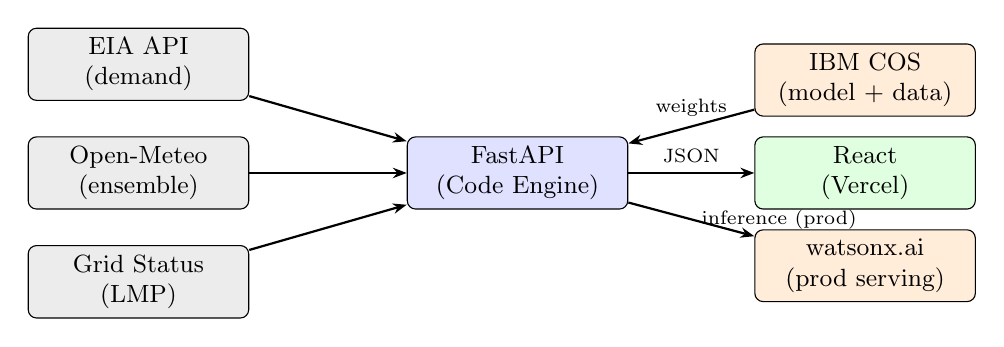
\begin{tikzpicture}[
  box/.style={rectangle, draw, rounded corners=3pt,
              minimum width=2.8cm, minimum height=0.85cm,
              font=\small, align=center},
  arr/.style={-{Stealth[length=5pt]}, thick},
  node distance=1.0cm and 1.8cm
]
  % Data sources (left column)
  \node[box, fill=gray!15]                        (eia) {EIA API\\(demand)};
  \node[box, fill=gray!15, below=0.45cm of eia]   (om)  {Open-Meteo\\(ensemble)};
  \node[box, fill=gray!15, below=0.45cm of om]    (gs)  {Grid Status\\(LMP)};

  % Backend (centre)
  \node[box, fill=blue!12, right=2.0cm of om]     (api) {FastAPI\\(Code Engine)};

  % Storage + model (right of backend)
  \node[box, fill=orange!15, above right=0.25cm and 1.6cm of api] (cos) {IBM COS\\(model + data)};
  \node[box, fill=orange!15, below right=0.25cm and 1.6cm of api] (wxa) {watsonx.ai\\(prod serving)};

  % Frontend (far right)
  \node[box, fill=green!12, right=1.6cm of api]   (fe)  {React\\(Vercel)};

  % Arrows
  \draw[arr] (eia) -- (api);
  \draw[arr] (om)  -- (api);
  \draw[arr] (gs)  -- (api);
  \draw[arr] (cos) -- (api) node[midway, above, font=\scriptsize] {weights};
  \draw[arr] (api) -- (wxa) node[midway, right, font=\scriptsize] {inference (prod)};
  \draw[arr] (api) -- (fe)  node[midway, above, font=\scriptsize] {JSON};
\end{tikzpicture}
\caption{GridCast system architecture. Arrows show data flow at inference time.}
\label{fig:arch}
\end{figure}

\subsection{API Endpoints}

\begin{table}[H]
\centering
\caption{Backend API surface.}
\label{tab:api}
\renewcommand{\arraystretch}{1.25}
\begin{tabularx}{\linewidth}{@{}llX@{}}
\toprule
\textbf{Method} & \textbf{Path} & \textbf{Description} \\
\midrule
GET  & \texttt{/nodes}                       & List of 4 nodes with current
                                               stress colour and allocation \% \\
GET  & \texttt{/nodes/\{id\}/forecast}       & 10-day quantile forecast as JSON
                                               (5 quantiles $\times$ 240 hours) \\
GET  & \texttt{/nodes/\{id\}/live}           & Latest EIA snapshot +
                                               Open-Meteo ensemble summary \\
POST & \texttt{/nodes/\{id\}/refresh}        & Pull fresh data and rerun
                                               inference; returns updated forecast \\
GET  & \texttt{/replay/\{event\_id\}}        & Pre-computed backtest output for
                                               a named historical stress event \\
\bottomrule
\end{tabularx}
\end{table}

% ============================================================
\section{Build Sequence}

The build is organised into seven phases. Phases 1a--1d and Phase~6 can run in parallel
once Phase~0 is complete. Phase~3 (training) is the longest serial step and blocks
Phase~4.

\begin{table}[H]
\centering
\caption{Phased build sequence with dependencies.}
\label{tab:phases}
\renewcommand{\arraystretch}{1.3}
\begin{tabularx}{\linewidth}{@{}llXl@{}}
\toprule
\textbf{Phase} & \textbf{Name} & \textbf{Tasks} & \textbf{Blocks} \\
\midrule
0 & Accounts \& Keys
  & IBM Cloud free trial; IBM COS bucket; Code Engine project;
    watsonx.ai project; EIA API key; Mapbox token; CDS account
  & Everything \\
\midrule
1a & ERA5 download
   & \texttt{cdsapi}: 2\,m temp, 10\,m wind, solar radiation; bounding
     boxes around 4 nodes; 2020--2024; upload to COS
   & Phase~2 \\
1b & EIA pipeline
   & \texttt{requests}: PJM / CISO / ERCO demand + fuel-type
     data 2020--2024; upload to COS
   & Phase~2 \\
1c & LMP pipeline
   & \texttt{gridstatus}: Dominion Hub, SP15, NP15, Houston Hub;
     real-time + day-ahead 2020--2024; upload to COS
   & Phase~2 \\
1d & Merge \& align
   & Resample all sources to hourly UTC; join on timestamp + node;
     output one Parquet per node to COS
   & Phase~2 \\
\midrule
2 & Feature engineering
  & Demand deviation; renewable penetration; LMP z-score; solar
    ramp rate; demand/capacity ratio; cyclical time encoding
  & Phase~3 \\
\midrule
3 & Model training
  & \tft on Colab T4 GPU; encoder 168\,h, decoder 240\,h; quantiles
    [0.1, 0.25, 0.5, 0.75, 0.9]; validate on 3 stress events;
    serialise \texttt{.ckpt}; upload to COS
  & Phase~4 \\
\midrule
4 & Backend API
  & FastAPI; loads weights from COS; calls EIA + Open-Meteo;
    runs \tft inference; 5 endpoints; Dockerfile
  & Phase~5 \\
\midrule
5 & IBM deployment
  & Push image to IBM Container Registry; deploy Code Engine
    application; set env vars; register model in watsonx.ai
    deployment space
  & Phase~7 \\
\midrule
6 & Frontend
  & React + Mapbox GL JS (map); Recharts (fan chart); node
    panel with allocation \%; data centre overlays; replay mode;
    deploy on Vercel
  & Phase~7 \\
\midrule
7 & Integration
  & Wire frontend to Code Engine URL; test all 4 nodes end-to-end;
    validate replay for Texas 2021; add IBM badge
  & Demo \\
\bottomrule
\end{tabularx}
\end{table}

\paragraph{Critical path.}
Phase~0 $\to$ \{1a, 1b, 1c\} in parallel $\to$ 1d $\to$ 2 $\to$ 3 $\to$ 4 $\to$ 5 $\to$ 7.
Phase~6 (frontend) can be built with mocked JSON responses while Phases 3--5 are
in progress.

% ============================================================
\section{Technology Stack Summary}

\begin{table}[H]
\centering
\caption{Full technology stack.}
\label{tab:stack}
\renewcommand{\arraystretch}{1.25}
\begin{tabularx}{\linewidth}{@{}llX@{}}
\toprule
\textbf{Layer} & \textbf{Technology} & \textbf{Notes} \\
\midrule
Weather (demo)     & Open-Meteo Ensemble API   & Free, no key, 16-member GFS ensemble \\
Weather (prod)     & \gencast / \graphcast     & Google DeepMind open weights; requires GPU/TPU \\
Grid demand        & EIA API v2                & Free, API key required \\
Nodal LMP          & \texttt{gridstatus}       & Free tier for recent data \\
Historical weather & ERA5 via \texttt{cdsapi}  & Free, CDS account required \\
\midrule
ML model           & PyTorch Forecasting \tft  & Quantile regression, multi-horizon \\
Training           & Google Colab (T4 GPU)     & Free tier sufficient for 4-node dataset \\
\midrule
Backend            & FastAPI + Python 3.11     & Containerised via Docker \\
Hosting            & IBM Cloud Code Engine     & Serverless; free trial \\
Storage            & IBM Cloud Object Storage  & Model artefacts + processed data \\
Model serving      & watsonx.ai                & Production path; registered in demo pitch \\
Container image    & IBM Container Registry    & Free tier \\
\midrule
Frontend           & React + Vite              & \\
Map                & Mapbox GL JS              & Free tier: 50k loads/month \\
Charts             & Recharts                  & Fan chart for quantile bands \\
Styling            & Tailwind CSS              & \\
Deploy             & Vercel                    & Free tier \\
\bottomrule
\end{tabularx}
\end{table}

% ============================================================
\appendix
\section{Updated Data Sources}

\subsection{Open-Meteo Ensemble API}

\textbf{Source:} \url{open-meteo.com}. Free, no API key required. Provides a
16-member GFS ensemble (\texttt{gfs\_seamless} model) at hourly resolution up to
16~days ahead. Variables used: \texttt{temperature\_2m}, \texttt{wind\_speed\_10m},
\texttt{shortwave\_radiation}. The ensemble spread across 16~members provides the
uncertainty signal that propagates through the \tft as known future covariates.

\begin{lstlisting}[language=bash,
  caption={Open-Meteo ensemble query for Dominion Hub (Northern Virginia).}]
GET https://ensemble-api.open-meteo.com/v1/ensemble
  ?latitude=38.9&longitude=-77.0
  &hourly=temperature_2m,wind_speed_10m,shortwave_radiation
  &models=gfs_seamless
  &forecast_days=10
\end{lstlisting}

\subsection{EIA, Grid Status, ERA5}

Unchanged from the original proposal Appendix~A. EIA API~v2 remains the source for
regional demand and fuel-mix data. The \texttt{gridstatus} Python library remains the
source for nodal LMP. ERA5 via \texttt{cdsapi} remains the historical weather ground
truth for training.

\end{document}
